% REVISÃO DE LITERATURA-------------------------------------------
\chapter{DISPOSITIVOS LÓGICOS E LÓGICA PROGRAMÁVEL}
\label{cap2}


\begin{figure}[!htb]
    \centering
    \caption{A estrutura de uma descrição VHDL com os seus blocos}
    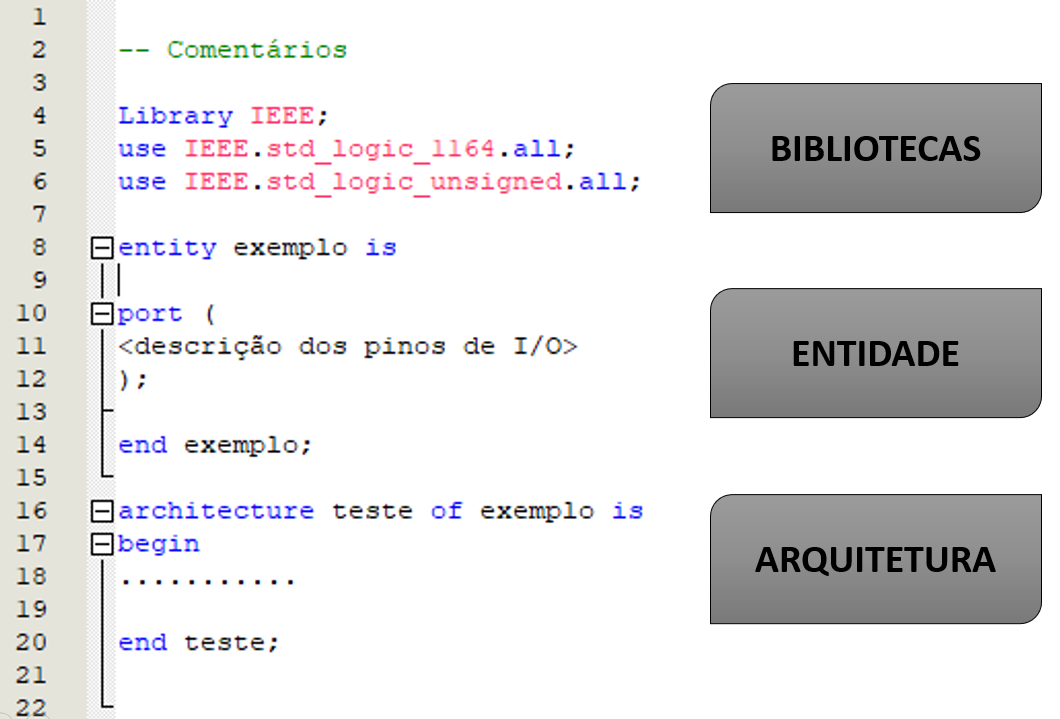
\includegraphics[height = 9cm]{figuras/estrut_blocVHDL.png}\\
    {\footnotesize Fonte: Autoria própria.}
    \label{fig:vhdl_blocos_estrut}
\end{figure}
 
\subsubsection{Declaração de biblioteca e Pacotes}

As bibliotecas e os pacotes são conjuntos de declarações usadas para um determinado fim. Pode ser um conjunto de subprogramas, ou funções que operem com um tipo de dado, assim como pode ser um conjunto de declarações necessárias para modelar um determinado projeto. Uma biblioteca é usada para organizar e gerenciar diferentes unidades de design em um projeto VHDL. É comum criar diferentes bibliotecas para organizar e armazenar unidades de design relacionadas. Por exemplo, uma biblioteca pode ser criada para armazenar unidades de design relacionadas a interface serial, enquanto outra biblioteca pode ser criada para armazenar unidades de design relacionadas a processamento de sinais \cite{roth2004circuit}.

Os pacotes são usados para definir e compartilhar constantes, tipos de dados, funções, procedimentos e outras construções que podem ser usadas em várias unidades de design. Os pacotes podem ser usados para evitar a repetição de código e facilitar a reutilização de código em diferentes unidades de design \cite{ordonez2003projeto}. Por exemplo, um pacote pode ser criado para definir um tipo de dado personalizado que é usado em várias unidades de design. 
Bibliotecas e Pacotes mais utilizados estão citados no quadro \ref{quadro_1}.
%+++++++++++++++++++++++++++++++++++++++++++++++

\begin{quadro}[h]
    \caption{Pacotes mais utilizados (Biblioteca IEEE)}
    \label{quadro_1}
    \centering
     \begin{tabular}{|c|p{3cm}|p{8cm}|}
      \hline
      \textbf{Pacote} & \textbf{Tipos de dados} & \textbf{Descrição} \\
      \hline
      std\_logic & std\_logic e std\_logic\_vector & Define o padrão para descrever a interconexão entre tipos de dados usados na linguagem VHDL \\
      \hline
       std\_logic\_arith & Especifica tipos de dados sinalizados e não sinalizados & Funções de conversão, operações aritméticas e comparações para uso de dados sinalizados e não sinalizados \\
      \hline
       std\_logic\_unsigned & std\_logic\_vector & Define funções que permitem usar tipos de dados std\_logic\_vector, como se fossem tipo de dado não sinalizado \\
      \hline
       std\_logic\_signed & std\_logic\_vector & Define funções que permitem usar tipos de dados std\_logic\_vector, como se fossem tipo de dado sinalizado \\
      \hline
       numeric\_std & & Substitui os pacotes usados juntos std\_logic\_atith, std\_logic\_unsigned e std\_logic\_signed \\
      \hline                 
    \end{tabular}
  \vspace{1.5pt}
  \caption*{\footnotesize Fonte: \cite{ordonez2003projeto}}
\end{quadro}

A declaração do uso de pacotes e bibliotecas é mostrada no quadro \ref{quadro_2}. O uso de .all implica que todos os elementos da biblioteca podem ser usados.


\subsubsection{Declaração de Entidade}

\begin{table}[htb]
\ABNTEXfontereduzida
\center \caption{Parâmetros da Condutividade Intrabanda do Grafeno \cite{b5}\cite{b13}}
\label{Tab1}
\vline  \begin{tabular}{p{0.6cm}|p{2cm}|p{2cm}|p{6cm}}
  \hline
   \textbf{ } & \textbf{Valor}  & \textbf{Unidade}  & \textbf{Descrição}  \\
   \hline
	\hline
$e$  &  $1,60\times10^{-19}$  &   $C$  &    Carga do Elétron\\
$\hbar$   &   $1,05\times10^{-34}$ & $J\!\cdot\!s/rad $ & Constante de Plank Reduzida\\
$k_B$   &   $1,38\times10^{-23}$ & $J/K $ & Constante de Boltzmanm\\
$T$   &   $300$ & $K$ &  Temperatura\\
$\sigma_0$   &   $e^2/4\hbar$ & $S\!\cdot\!rad$ & Condutividade HF\\
$\mu_c$   &   $0; 0,25; 0,5$ & $eV$ & Potencial Químico\\
$\tau$   &   $0,5$ & $ps$ & Tempo de Amortecimento\\
\hline

\end{tabular}\vline  
\end{table}

\begin{equation}\label{eq3.2}
\textbf{E}_1(x,z) = -\hat{a}_y\left[E_{iy}e^{-jk_{z1}(z+d_1)} + E_{ry}e^{+jk_{z1}(z+d_1)}\right]e^{-jk_x x}  
\end{equation}